% ---------------------------------------------------------------------------
\section{New points in the space}
\label{sec:generative}

Coding existing techniques shows what the model can \emph{describe}. Its
\emph{generative} power~\cite{beaudouinlafon2004designing} is the other half:
whether it reaches configurations that were not built before, by changing
arguments rather than by writing new techniques. \Cref{fig:gallery} shows
eighteen configurations of one implementation on one dataset---1{,}449
OpenStreetMap places in central Yogyakarta, in four categories---each captioned
with its path through the stages. We discuss the ones we believe are new,
grouped by the stage that makes them possible.
\doubt{``New'' means: not found in the literature reviewed for
\cref{sec:related}. Keep this wording until a systematic search (with a
recorded protocol) backs a stronger one.}

\begin{figure*}[t]
  \centering
  \newcommand{\tile}[2]{%
    \begin{subfigure}[t]{0.158\textwidth}\centering
      \includegraphics[width=\linewidth]{figures/#1}\caption*{\scriptsize #2}
    \end{subfigure}}
  \tile{g-category-ring}{(a) categorical, block}\hfill
  \tile{g-necklace}{(b) categorical, necklace}\hfill
  \tile{g-compass}{(c) angular(24)}\hfill
  \tile{g-spread}{(d) + spread}\hfill
  \tile{g-rose}{(e) rose marks}\hfill
  \tile{g-disc}{(f) disc marks}\\[2pt]
  \tile{g-stacked}{(g) cross(8), stacked}\hfill
  \tile{g-lq}{(h) location quotient}\hfill
  \tile{g-radial}{(i) radial(5), density}\hfill
  \tile{g-polygon}{(j) polygon selection}\hfill
  \tile{g-corridor}{(k) corridor, chainage}\hfill
  \tile{g-block-leader}{(l) block + leaders}\\[2pt]
  \tile{g-unroll}{(m) unrolled ring}\hfill
  \tile{g-upright}{(n) upright marks}\hfill
  \tile{g-corridor-unroll}{(o) corridor, unrolled}\hfill
  \tile{g-unroll-leader}{(p) unrolled + leaders}\hfill
  \tile{g-relaxed}{(q) relaxed lattice}\hfill
  \tile{g-inclusions}{(r) + inclusions}
  \caption{Eighteen configurations of one pipeline on one dataset (1{,}449
  OpenStreetMap places, central Yogyakarta, four categories), rendered by the
  library on bare canvases with no map. (a) is the category ring common in lens
  demonstrations: angle carries category order. (b) is the same four bins placed
  at their members' mean bearing. (c)--(f) bin by bearing sector and vary the
  mark and within-unit encoding. (g)--(k) vary binning, normalisation and
  selection. (l)--(p) vary the anchor and association. (q) is a field on a
  relaxed lattice inside a concave boundary; (r) draws the members back through
  their aggregates. Paths through the stages are given in the text and in the
  repository's gallery.}
  \label{fig:gallery}
\end{figure*}

\paragraph{Angle as bearing.} Binning by bearing sector and placing each
sector's mark at its bearing (\cref{fig:gallery}c,f) turns a ring from a legend
into a compass: a mark at eleven o'clock means the data it summarises lies to
the north-west. The same move applied to categorical bins
(\cref{fig:gallery}a$\to$b) interpolates, with one parameter, from the familiar
category ring to a bearing-faithful one; the transition is a lerp of preferred
positions through the same solver. As \cref{sec:discussion} discusses, the
categorical version is honest only for segregated categories, and crossing
bearing with category (\cref{fig:gallery}g) is the robust form.

\paragraph{The anchor as an axis.} Because placement is solved in the curve's
parameter and holds length constant, the ring unrolls into a straight axis with
no re-solve (\cref{fig:gallery}m), and a corridor straightens onto its own
chainage in exactly the same way (\cref{fig:gallery}k$\to$o). The unrolled ring
is a bar chart with bearing on the horizontal axis---comparable lengths, room
for labels---and it is a strip, so several lenses can share one baseline. Upright
marks on a closed ring (\cref{fig:gallery}n) buy some of the same comparability
without leaving the map.

\paragraph{Association as a residual.} Leaders appear exactly where adjacency
has been given away: under block placement, where every mark is far from its
data (\cref{fig:gallery}l), and under unrolling, where the whole chart has left
the map (\cref{fig:gallery}p). They are drawn to the members' mean position in
the lens's own frame, so their length is the association lost.

\paragraph{Within-unit structure from the lens's own geometry.} The spread arc
(\cref{fig:gallery}d) draws each category's circular standard deviation, so a
bar whose direction is not worth believing says so; rose marks
(\cref{fig:gallery}e) replace the mark with its full angular distribution; and
inclusions (\cref{fig:gallery}r) put the members back through the aggregate. On a
corridor the same layer becomes lateral: bias and sidedness of member offsets.

\subsection{The continuum from lens to glyphmap}
\label{sec:continuum}

Treating the number of lenses as a parameter gives a path from focus+context to
small multiples to a gridded glyphmap (\cref{fig:continuum}). The field is not a
second implementation: it calls the single-lens pipeline once per lattice centre
and shares one baseline across all of them. Its lattice is itself an axis
(hexagonal, square, triangular, or relaxed inside a boundary; \cref{fig:gallery}q),
with a measurable consequence for how much ground the lenses reach
(\cref{sec:discussion}).

Two findings from building it are worth stating. A field needs \emph{one}
baseline: a location quotient computed against each lens's own surroundings
makes every cell average by construction, so the map says nothing. And the
continuum has a usable range rather than an infinite one: as rings shrink the
renderer sheds labels, then compass, and at the dense end the field reads as a
surface (\cref{fig:continuum}, right).

The tessellated end is not new---it is the gridded
glyphmap~\cite{slingsby2018tilemaps,slingsby2023gridded,laksono2024gridded}, and
earlier tilemap work already proposed interactively resizing and panning the
grid to expose the modifiable areal unit problem, and smoothing with a
distance-decay kernel larger than the tiles~\cite{slingsby2018tilemaps}. What
the model adds is that the single lens, the small multiple and the glyphmap are
one object whose every other stage---binning by bearing, placement,
association, within-unit structure---survives the change of count.

\begin{figure*}[t]
  \centering
  \begin{subfigure}[t]{0.24\textwidth}\centering
    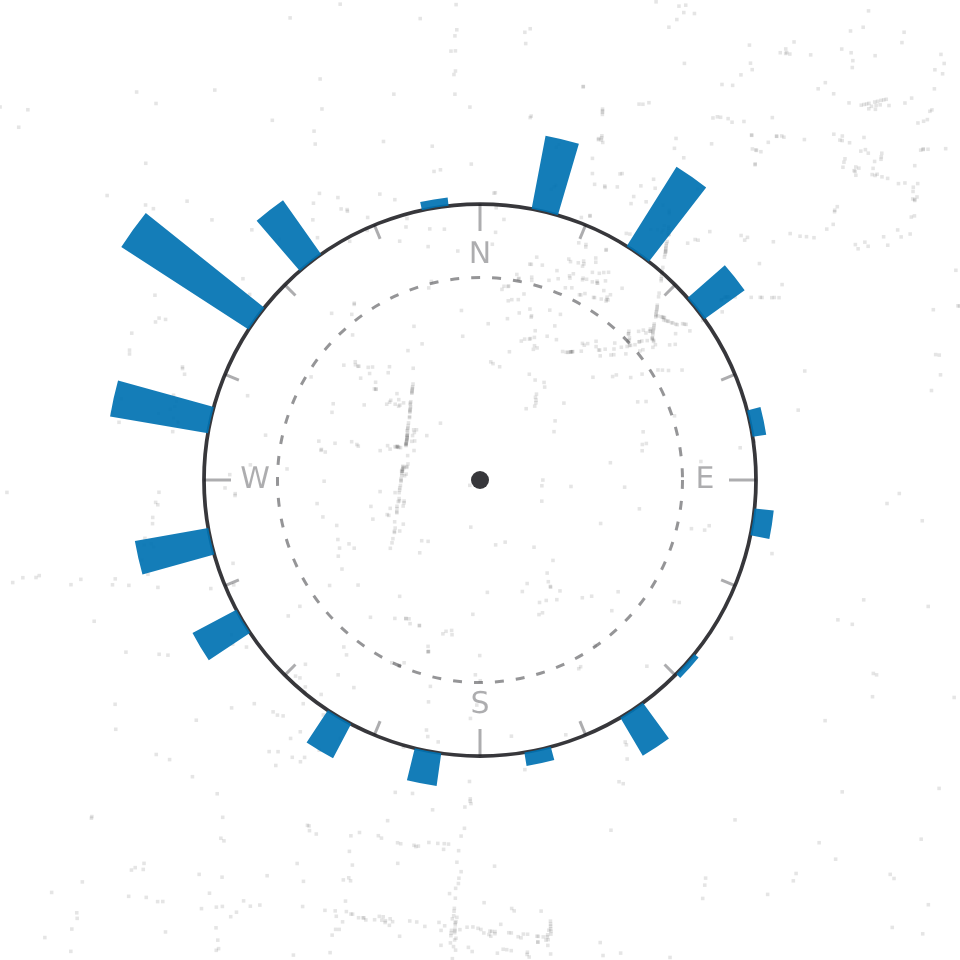
\includegraphics[width=\linewidth]{figures/c-continuum-1}\caption*{\small 1 lens}
  \end{subfigure}\hfill
  \begin{subfigure}[t]{0.24\textwidth}\centering
    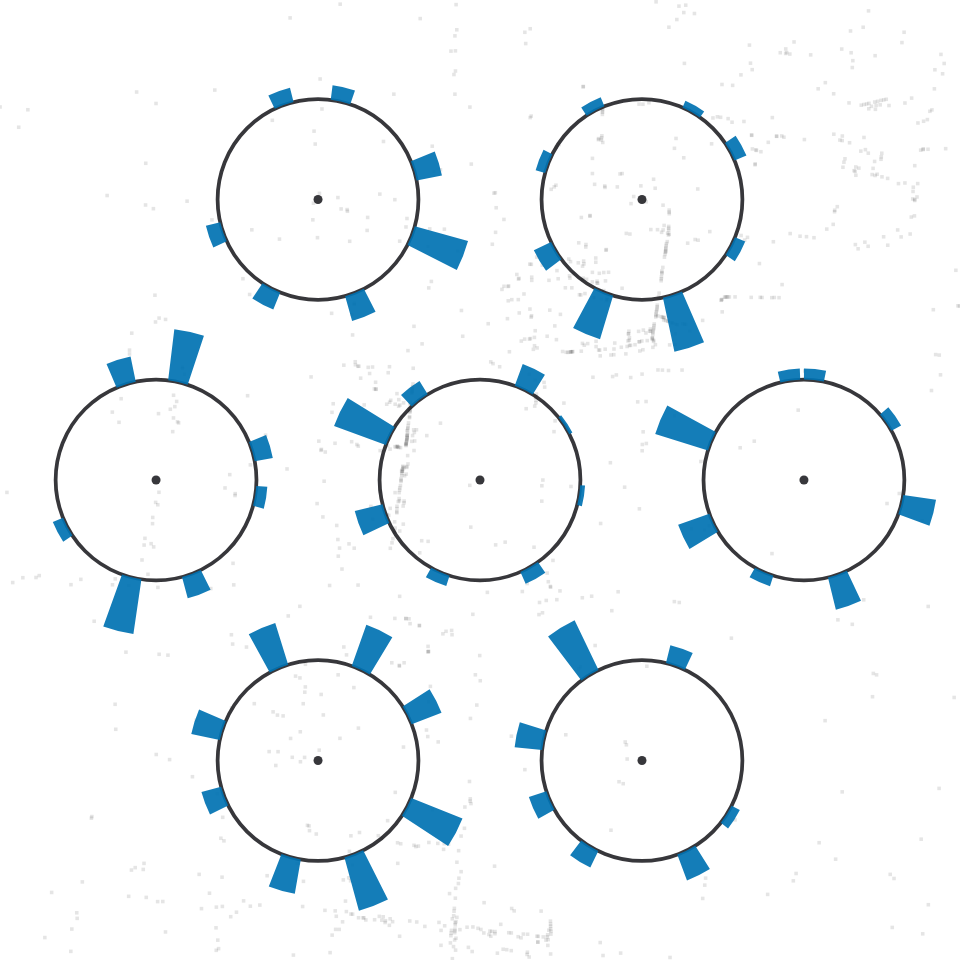
\includegraphics[width=\linewidth]{figures/c-continuum-7}\caption*{\small 7 lenses}
  \end{subfigure}\hfill
  \begin{subfigure}[t]{0.24\textwidth}\centering
    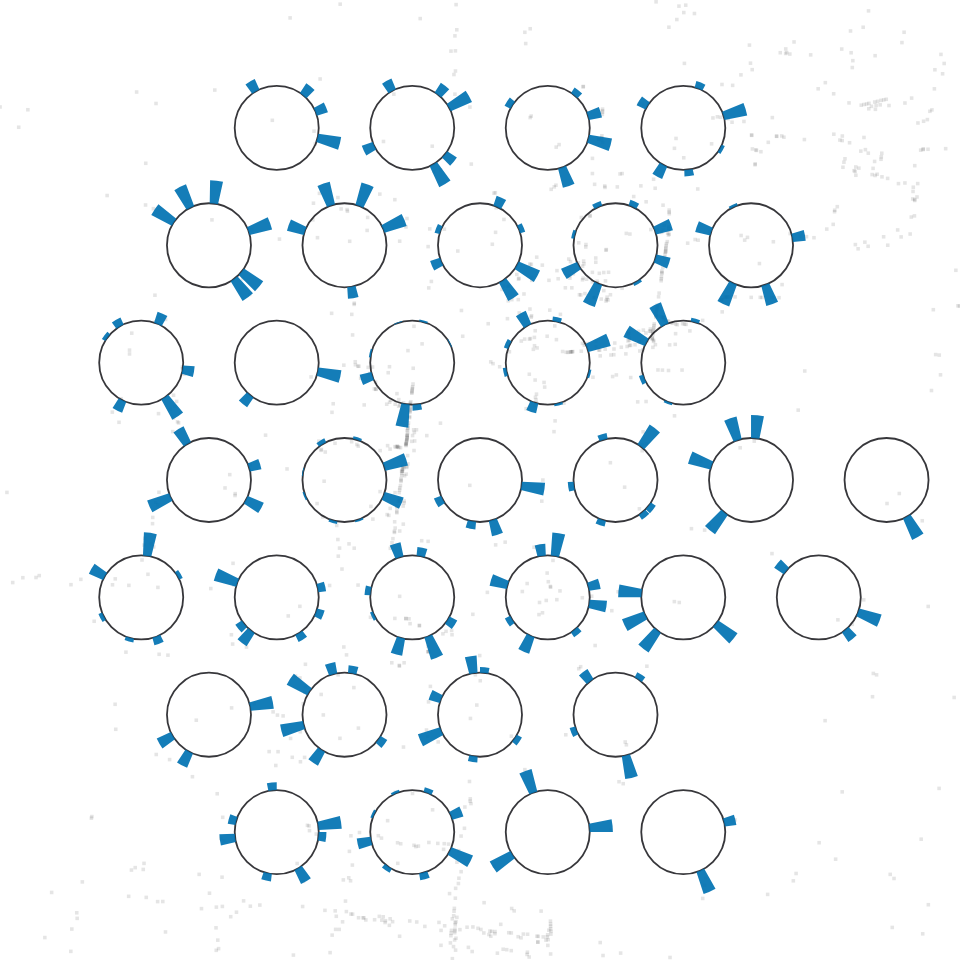
\includegraphics[width=\linewidth]{figures/c-continuum-40}\caption*{\small 37 lenses}
  \end{subfigure}\hfill
  \begin{subfigure}[t]{0.24\textwidth}\centering
    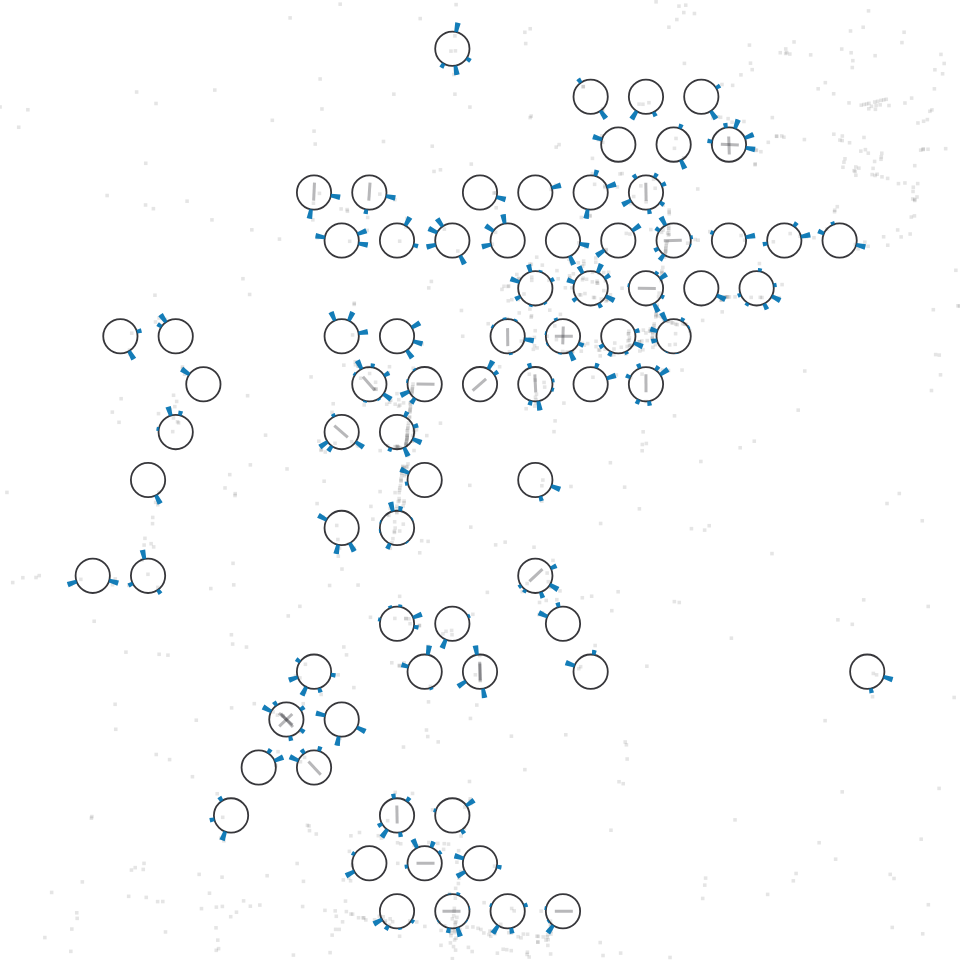
\includegraphics[width=\linewidth]{figures/c-continuum-240}\caption*{\small 241 lenses}
  \end{subfigure}
  \caption{One parameter---the number of lattice centres---takes a single
  bearing-faithful lens to a gridded glyphmap. Every panel is the same binning
  (bearing sectors), the same solver and the same renderer; only the lattice
  changes. Lenses with fewer than three members are not drawn. Grey dots are
  the members.}
  \label{fig:continuum}
\end{figure*}
